\section{Design}

\subsection{Database Design}
The project should have a database to store data. 
The data that should be stored in the database is a batch. 
You can see how the data should be stored in / 
configured in the databse in figure \ref{figure:eer_diagram_batch}.
The data is useful for making a completesystem for Refslevbæk Bryghus A/S, 
then they can make sure to have data about the batch they made. 

The Batch's database is used in the system to keep track of batch's.
For example if a person would like to know what happened then the beer got produced,
like what temperature was it then the temperature was highest, Did that ruin it.
How much was defect out of the totalt amount produced. 

\begin{figure}[ht]
\centering 
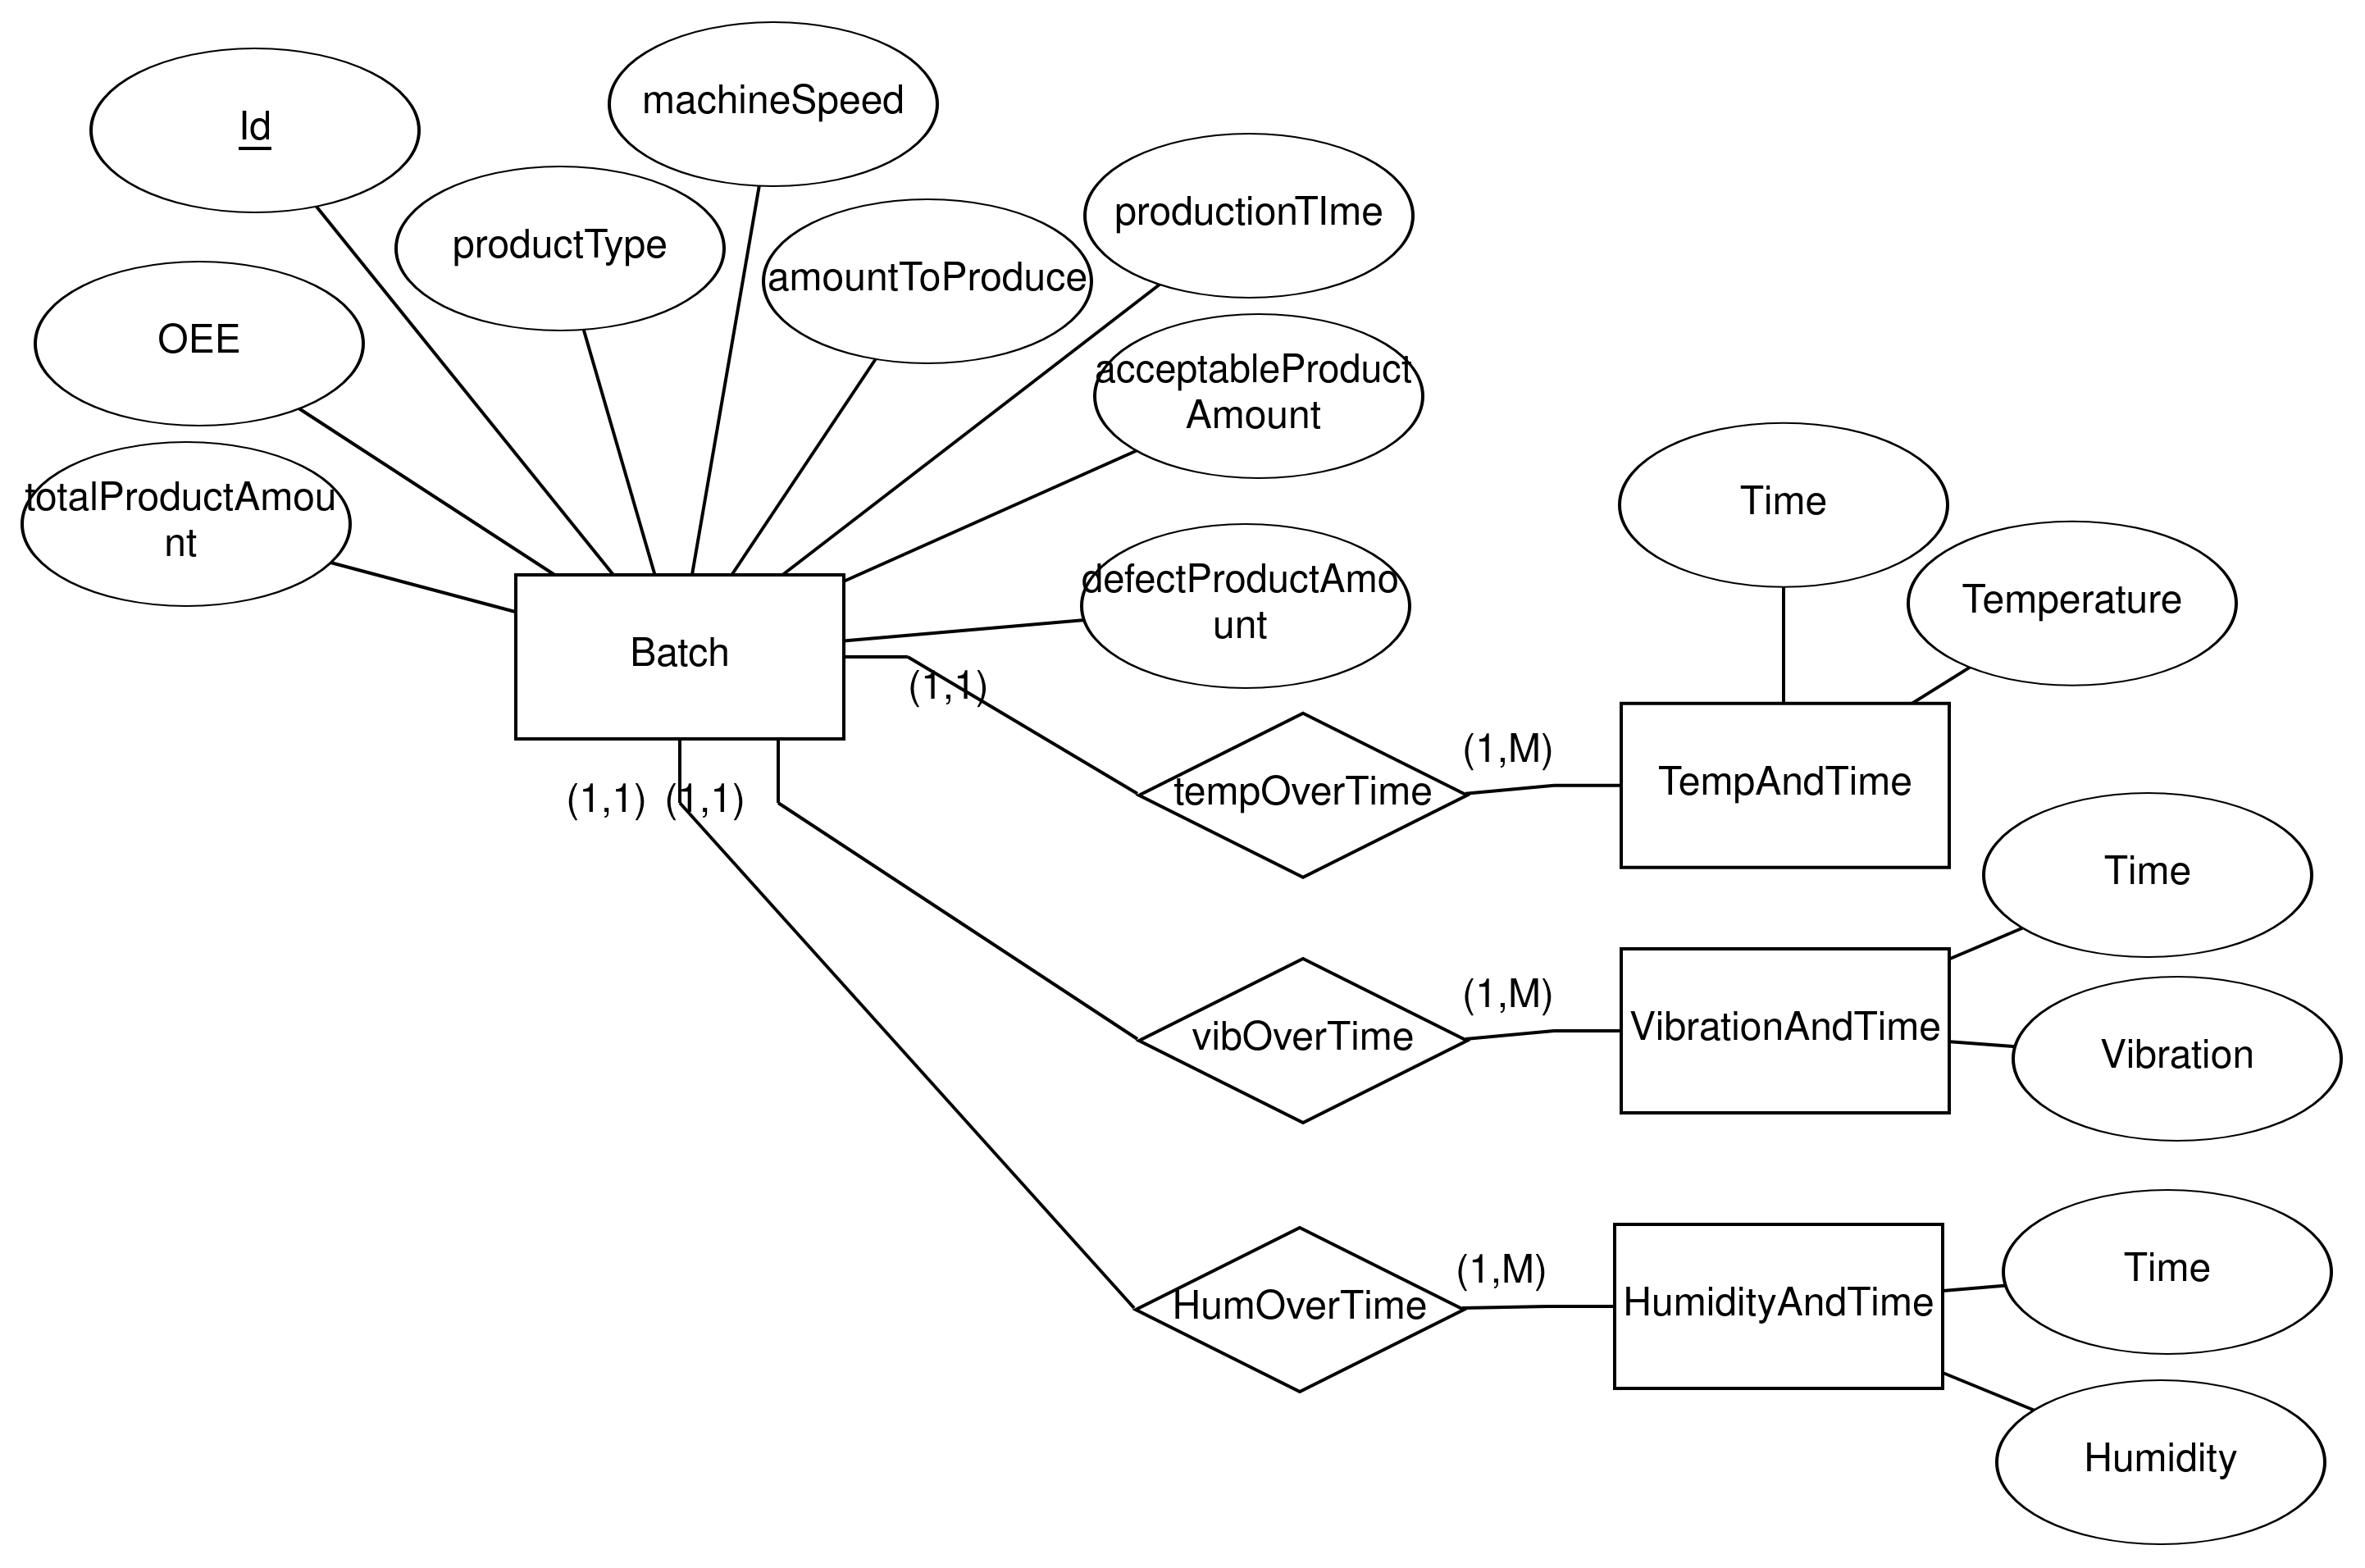
\includegraphics[width=0.8\linewidth]{images/eer_diagrams/database_EER_batch.png}
\caption{IR diagram for batch} 
\label{figure:eer_diagram_batch}
\end{figure}
